

% This is a small sample LaTeX input file (Version of 10 April 1994)
%
% Use this file as a model for making your own LaTeX input file.
% Everything to the right of a  %  is a remark to you and is ignored by LaTeX.

% The Local Guide tells how to run LaTeX.

% WARNING!  Do not type any of the following 10 characters except as directed:
%                &   $   #   %   _   {   }   ^   ~   \

%%%%%%%%%%%%%%%%%%%%%%% file typeinst.tex %%%%%%%%%%%%%%%%%%%%%%%%%
%
% This is the LaTeX source for the instructions to authors using
% the LaTeX document class 'llncs.cls' for contributions to
% the Lecture Notes in Computer Sciences series.
% http://www.springer.com/lncs       Springer Heidelberg 2006/05/04
%
% It may be used as a template for your own input - copy it
% to a new file with a new name and use it as the basis
% for your article.
%
% NB: the document class 'llncs' has its own and detailed documentation, see
% ftp://ftp.springer.de/data/pubftp/pub/tex/latex/llncs/latex2e/llncsdoc.pdf
%
%%%%%%%%%%%%%%%%%%%%%%%%%%%%%%%%%%%%%%%%%%%%%%%%%%%%%%%%%%%%%%%%%%%

\documentclass[conference]{IEEEtran}

%% INFOCOM 2011 addition:
\makeatletter
\def\ps@headings{%
\def\@oddhead{\mbox{}\scriptsize\rightmark \hfil \thepage}%
\def\@evenhead{\scriptsize\thepage \hfil \leftmark\mbox{}}%
\def\@oddfoot{}%
\def\@evenfoot{}}
\makeatother
\pagestyle{headings}
%\usepackage{latex8}
\usepackage{setspace}
\usepackage{times}
%\usepackage{kbordermatrix}% http://www.hss.caltech.edu/~kcb/LaTeX.shtml
\newcommand{\noindex}{\hspace*{-0.8em}}%
\usepackage{pgf}
\usepackage{tikz}
\usetikzlibrary{arrows,automata}
\usepackage[latin1]{inputenc}
\usetikzlibrary{arrows}
\usepackage{epsfig,xspace}
\usepackage{url}
\usepackage{verbatim}
\usepackage{amsmath}
\usepackage{listings}
\usepackage{verbatim}

\usepackage{graphicx}
\usepackage{epstopdf}
\usepackage{mathtools}
%\usepackage{fix2col}
\usepackage{multirow}
\usepackage{varwidth}
\usepackage{algorithm}
\usepackage{algorithm}
\usepackage{algpseudocode}
%\usepackage[dvips]{graphicx}
%\usepackage{mss}
%\usepackage{subfigure}
\usepackage{subfigure}
%\usepackage{nopageno}
%\usepackage{fix2col}
%\usepackage{authblk}
%\usepackage[pdfborder={0 0 0}]{hyperref}% For email addresses

\IEEEoverridecommandlockouts
\IEEEpubid{\makebox[\columnwidth]{978-1-4799-5671-5/14/\$31.00~\copyright2014
IEEE \hfill} \hspace{\columnsep}\makebox[\columnwidth]{ }}

\lstset{
  basicstyle=\footnotesize,
  columns=flexible,
  morecomment=[s]{/*}{*/}}

\newtheorem{Theorem}{Theorem}[section]
\newtheorem{lemma}[Theorem]{Lemma}
\newtheorem{proposition}[Theorem]{Proposition}
\newtheorem{corollary}[Theorem]{Corollary}

\newcommand{\remove}[1]{ }
\newcommand{\eg}{\emph{e.g.}}
\newcommand{\ie}{\emph{i.e.}}

\newenvironment{proof}[1][Proof:]{\begin{trivlist}
\item[\hskip \labelsep {\bfseries #1}]}{\end{trivlist}}


\newenvironment{definition}[1][Definition]{\begin{trivlist}
\item[\hskip \labelsep {\bfseries #1}]}{\end{trivlist}}
\newenvironment{example}[1][Example]{\begin{trivlist}
\item[\hskip \labelsep {\bfseries #1}]}{\end{trivlist}}
\newenvironment{remark}[1][Remark]{\begin{trivlist}
\item[\hskip \labelsep {\bfseries #1}]}{\end{trivlist}}

\renewcommand{\algorithmicrequire}{\textbf{Input:}}
\renewcommand{\algorithmicensure}{\textbf{Output:}}

\newcommand{\qed}{\nobreak \ifvmode \relax \else
      \ifdim\lastskip<1.5em \hskip-\lastskip
      \hskip1.5em plus0em minus0.5em \fi \nobreak
      \vrule height0.6em width0.5em depth0.0em\fi}

\def\sqzhuge{\vspace{-14pt}}
\def\sqzsec{\vspace{-10pt}}
\def\sqzsmall{\vspace{-8pt}}
\def\sqztiny{\vspace{-4pt}}
\remove{
\usepackage{vmargin}
\setpapersize{USletter}
\setmarginsrb{2.54cm}{2.54cm}{2.54cm}{1.5cm}{0pt}{0mm}{0pt}{8mm}
\setcounter{secnumdepth}{3}
}
\newcommand\Mark[1]{\textsuperscript#1}

\begin{document}
\pagenumbering{gobble}

\title{SSD-Optimized Workload Placement with Adaptive Learning and Classification in HPC Environments}
%\author{\IEEEauthorblockN{Lipeng Wan\IEEEauthorrefmark{1}, Zheng Lu\IEEEauthorrefmark{1}, Qing Cao\IEEEauthorrefmark{1}, Feiyi Wang\IEEEauthorrefmark{2}, Sarp Oral\IEEEauthorrefmark{2}, and Bradley Settlemyer\IEEEauthorrefmark{2}}\\
%\vspace{-0.1in}
%%\begin{tabular}{*{2}{>{\centering}p{.45\textwidth}}}
%\IEEEauthorblockA{\IEEEauthorrefmark{1}Department of Electrical Engineering and Computer Science\\University of Tennessee, Knoxville, TN, US\\
%Email: \{lwan1, zhenglu, cao\}@utk.edu} \\
%\vspace{-0.15in}
%\IEEEauthorblockA{\IEEEauthorrefmark{2}Oak Ridge National Laboratory\\ Oak Ridge, TN, US\\
%Email: \{fwang2, oralhs, settlemyerbw\}@ornl.gov}
%%\end{tabular}
%\vspace{-0.3in}
%}
\author{
    \IEEEauthorblockN{Lipeng Wan\IEEEauthorrefmark{1}, Zheng Lu\IEEEauthorrefmark{1}, Qing Cao\IEEEauthorrefmark{1}}
    \IEEEauthorblockA{
        \IEEEauthorrefmark{1}Department of Electrical Engineering and Computer Science\\
        University of Tennessee, Knoxville, TN, US\\
        Email: \{lwan1, zlu12, cao\}@utk.edu}
    \and
    \IEEEauthorblockN{Feiyi Wang\IEEEauthorrefmark{2}, Sarp Oral\IEEEauthorrefmark{2}, Bradley Settlemyer\IEEEauthorrefmark{2}}
    \IEEEauthorblockA{
        \IEEEauthorrefmark{2}Oak Ridge National Laboratory\\
        Oak Ridge, TN, US\\
        Email: \{fwang2, oralhs, settlemyerbw\}@ornl.gov}
}

\vspace{-0.8in}
\maketitle


\vspace{-1in}
\begin{abstract}


In recent years, non-volatile memory devices such as SSD drives have emerged
as a viable storage solution due to their increasing capacity and decreasing
cost. Due to the unique capability and capacity requirements in large scale
HPC (High Performance Computing) storage environment, a hybrid configuration
(SSD and HDD) may represent one of the most available and balanced solutions
considering the cost and performance. Under this setting, effective data
placement as well as movement with controlled overhead become a pressing
challenge. In this paper, we propose an integrated object placement and
movement framework and adaptive learning algorithms to address these issues.
Specifically, we present a method that shuffle data objects across storage
tiers to optimize the data access performance. The method also
integrates an adaptive learning algorithm where real-time classification is
employed to predict the popularity of data object accesses, so that they can
be placed on, or migrate between SSD or HDD drives in the most efficient
manner. We discuss preliminary results based on this approach using a
simulator we developed to show that the proposed methods can dynamically adapt
storage placements and access pattern as workloads evolve to achieve the best
system level performance such as throughput.

\end{abstract}

%\IEEEpeerreviewmaketitle


\section{Introduction}
\label{intro}

With the explosive increase in the amount of data being generated by various HPC applications, developing resilient and high-performance storage solutions becomes even more of a challenge \cite{lofstead2010managing,DBLP:conf/mss/ZhuWLHLM13}. Therefore, it is crucial to come up with effective data placement mechanisms in a heterogamous environment based on the nature of workloads, as well as the properties of the underlying hardware such as their network topology and bandwidth. On the other hand, both the workloads and the underlying hardware evolve over time, so it requires algorithms have to be designed to take these changes into their consideration.

One particular trend that has emerged in recent years is the use of SSD drives in storage solutions to provide \emph{premium} services, as the read and write speed for SSD drives are typically much faster compared to hard drives~\cite{park2009performance}. On the other hand, SSD drives have different failure patterns where repeated read and write operations of the same address blocks will cause the drives to fail~\cite{chen2009understanding}. Furthermore, SSD drives are also limited in capacity, meaning that it is not yet practical to use them to completely replace conventional hard disks. Therefore, how to effectively integrate SSD drives into the design of storage systems for HPC environments becomes a critical yet challenging task.

Existing algorithms to integrate SSD drives can already be found in the literature~\cite{DBLP:conf/mss/WangHHZLH13, DBLP:conf/mss/LeeKKLPM13}. These methods, while effective, are largely based on heuristic algorithms that are either developed in isolation with the runtime workload, or are based on static assumptions on the workload patterns, making them unsuitable when the underlying workloads and demands change over time.

To address such drawbacks, we present a holistic approach where we aim to develop a framework that adaptively classifies the popularity of data objects, adjusts their placement among storage tiers by moving them between slower HDDs and faster SSDs, and fulfills the needs of users with regard to their I/O operation requirements. Formally, our developed algorithm makes the following assumptions. First, we assume that the storage hardware consists of both slower HDD drives and faster SSD drives. Second, the user may have their own rules for the placement of data, such as, a particular data object must be stored on HDDs with three copies available for a certain period of time, among others. Therefore, such rules must be properly fulfilled during runtime.

Based on these assumptions, our proposed method makes two contributions: first, it proposes a Markov-chain based classification model to predict whether data objects will be accessed frequently in the future based on their historical access records; second, it develops an integrated data placement engine that is based on linear programming for fulfilling the requirements of throughput and reliability from the users.  We next describe these two contributions separately.

In the first contribution, we classify data objects based on their access patterns, including both their access frequencies and the particular workload that accessed them, so that we can determine those objects that are most likely to be accessed frequently in the future. Our method is based on training a Markov chain model, and once such predictions are made, we move
those frequently accessed objects to SSD drives under the constraint that the moving cost does not exceed the predicted savings.

In the second contribution, we consider the challenge on fulfilling the user policies on data placements, such as their preferences on where to place the objects. To this end, we develop a data placement engine that takes user policies and the performance variation between storage devices, such as the bandwidth and delays between two HDDs or SSDs, as input, and generates a satisfying solution, if any, as the output. The theoretical foundation of this engine stems from linear programming, where we allow numerical methods to be adopted to find solutions. For example, if the user specifies that no two
copies of a data object should be on the same rack, such a requirement will be formulated as a constrain in the linear programming model and be guaranteed in the solution.

%The key contributions of the developed algorithm are listed as follows: first, we present an access-frequency sensitive algorithm for extending the CRUSH algorithm. The core methodology involves modeling the different storage services based on their access latency parameters, and try to minimize the overall access time through an optimization problem.
%
%Second, we observe that given that users' request patterns change over time, it is time-consuming to re-solve the problem every time the user input changes. Therefore, we develop a learning algorithm to classify the input patterns, and generate the output parameters automatically after the training phase. This approach allows the extension of CRUSH to handle different application requirements highly efficiently.


The rest of this paper is organized as follows. We describe the related work in Section~\ref{sec:relatedwork}. The design is described in Section~\ref{sec:design}. The performance evaluation is given in Section~\ref{sec:evaluation}. We provide conclusions in Section~\ref{sec:conclusion}. %We survey related work in Section~\ref{sec:related}.

















\section{Related Work}
\label{sec:relatedwork}

In this section, we survey several existing works related to our paper. We classify these existing works into two categories. The first category consists of existing works on data placement algorithms for distributed storage systems, while the second consists of those on hybrid storage systems that aim to leverage SSD drives to improve data access performance.

As large-scale distributed storage systems have been extensively used in the HPC area, the problem of distributing several petabytes of data among hundreds or thousands of storage devices becomes more and more critical. To address this problem, many data placement algorithms have been proposed. For instance, Distributed Hash Tables (DHTs) have been used to place and locate data objects in P2P systems \cite{Stoica2001, Ratnasamy2001, Cai2004}. Another replica placement scheme called chain placement was also proposed and applied to some P2P and LAN storage systems \cite{Rowstron2001, Lee1996, MacCormick2004}. Honicky and Miller presented a family of algorithms named RUSH \cite{honicky04} that utilizes a mapping function to evenly map replicated
objects to a scalable collection of storage devices, so that it can support efficient additions and removals of weighted devices.

To address the reliability and replication issues of the RUSH algorithm, Weil et al. proposed a scalable pseudo-random data distribution algorithm named CRUSH \cite{Weil2006}. Besides optimally distributing data to available resources and efficiently reorganizing data after adding or removing storage devices, CRUSH exploits flexible constraints on replica placement to maximize data safety in the case of hardware failures. Specifically, CRUSH allows the administrator to assign different weights to storage devices so that the administrator can control the relative share of data each device is responsible for. However, the device weights used in the CRUSH algorithm only reflect the capacities of storage devices, therefore, the CRUSH algorithm may not be effective anymore for hybrid storage systems consisting of both SSD and HDD devices, as these two kinds of storage devices have totally different performance characteristics.

Recently, efforts have been made to combine SSD and HDD drives together to construct hybrid storage systems. In such systems, SSDs are either used for caching purposes, or used as more independent storage devices. For example, Srinivasan et al. designed a block-level cache named Flashcache \cite{Flashcache} between DRAM and hard disks using SSD devices. Zhang et al.
proposed iTransformer \cite{Zhang2012} which exploits a small SSD to schedule requests for the data on disks so that high disk efficiency can be achieved. SieveStore \cite{Pritchett2010} adopts a selective caching approach in which the accesses of each block are tracked and the most popular block is cached in SSD device. In the second approach, SSDs are more independently used. Chen et al. designed and implemented a high performance hybrid storage system named Hystor \cite{Chen2011}, which identifies data blocks that either can result in long latencies or are semantically critical on hard disks, and store them in SSDs for future accesses. In order to prolong the service life of SSDs devices, Ren et al. proposed I\_CASH \cite{Yang2011} to reduce random write traffic to SSDs. Specifically, I\_CASH is an approach that exploits the spacial locality of data accesses, and only store those seldom-changed data blocks on SSDs. Finally, ComboDrive \cite{Payer2009} concatenates SSD and HDD into one address space via a hardware-based solution, so that certain data on HDD can be moved into the faster SSD space.

There are two main differences between existing works on hybrid storage systems and our approach: first, most existing works on hybrid storage systems only consider how to improve the utilization of SSD drives, but they have ignored the reliability and replication issues in HPC environments; second, existing works have not considered the dynamic nature of workflows, a nature that makes continuous training and learning necessary. In our approach, we fully consider these issues, and our method provides up-to-date predictions on popular data blocks, so that we can store critical data on SSDs well in advance.

\section{Data Placement Algorithm Design}
\label{sec:design}

In this section, we introduce the design of the data placement algorithm. We first present the problem formulation. Then, we present an overview of our algorithm architecture. Finally, we present a detailed description of its components and related algorithms.


\subsection{Problem Formulation}
\label{problemformulation}

The core problem is formulated as follows. Given a set of storage devices represented by HDDs and SSDs as the hardware platform, our task is to find a data placement that 1) satisfies user polices on data placements, and 2) maximizes the throughput of I/O operations from HPC applications. This problem is challenging due to: 1) we don't have complete knowledge on future access patterns to data objects due to the dynamics of workloads, 2) user policies can be highly heterogeneous and may change over time. Therefore, if we model such a problem as an optimization problem, its solution is from a very large search space, such that it is very hard to always reach the optimal configuration when something changes, even such change could be slight. Furthermore, given that the users' request may change frequently, we would like to be able to re-use previous calculation results as much as possible, so that we can avoid the re-calculation when a similar scenario is met in practice.


%ased on such concerns, we formulate the following problem: \textbf{given the underlying demands, how can we find an optimized storage placement that can incrementally provide results that can achieve the best performance under the resource constraints and user requirements?} Note that given that the users' request may change frequently, we would like to be able to re-use previous calculation results as much as possible, so that we can avoid the re-calculation when a similar scenario is met in practice.

\begin{figure}[t]
\begin{centering}
  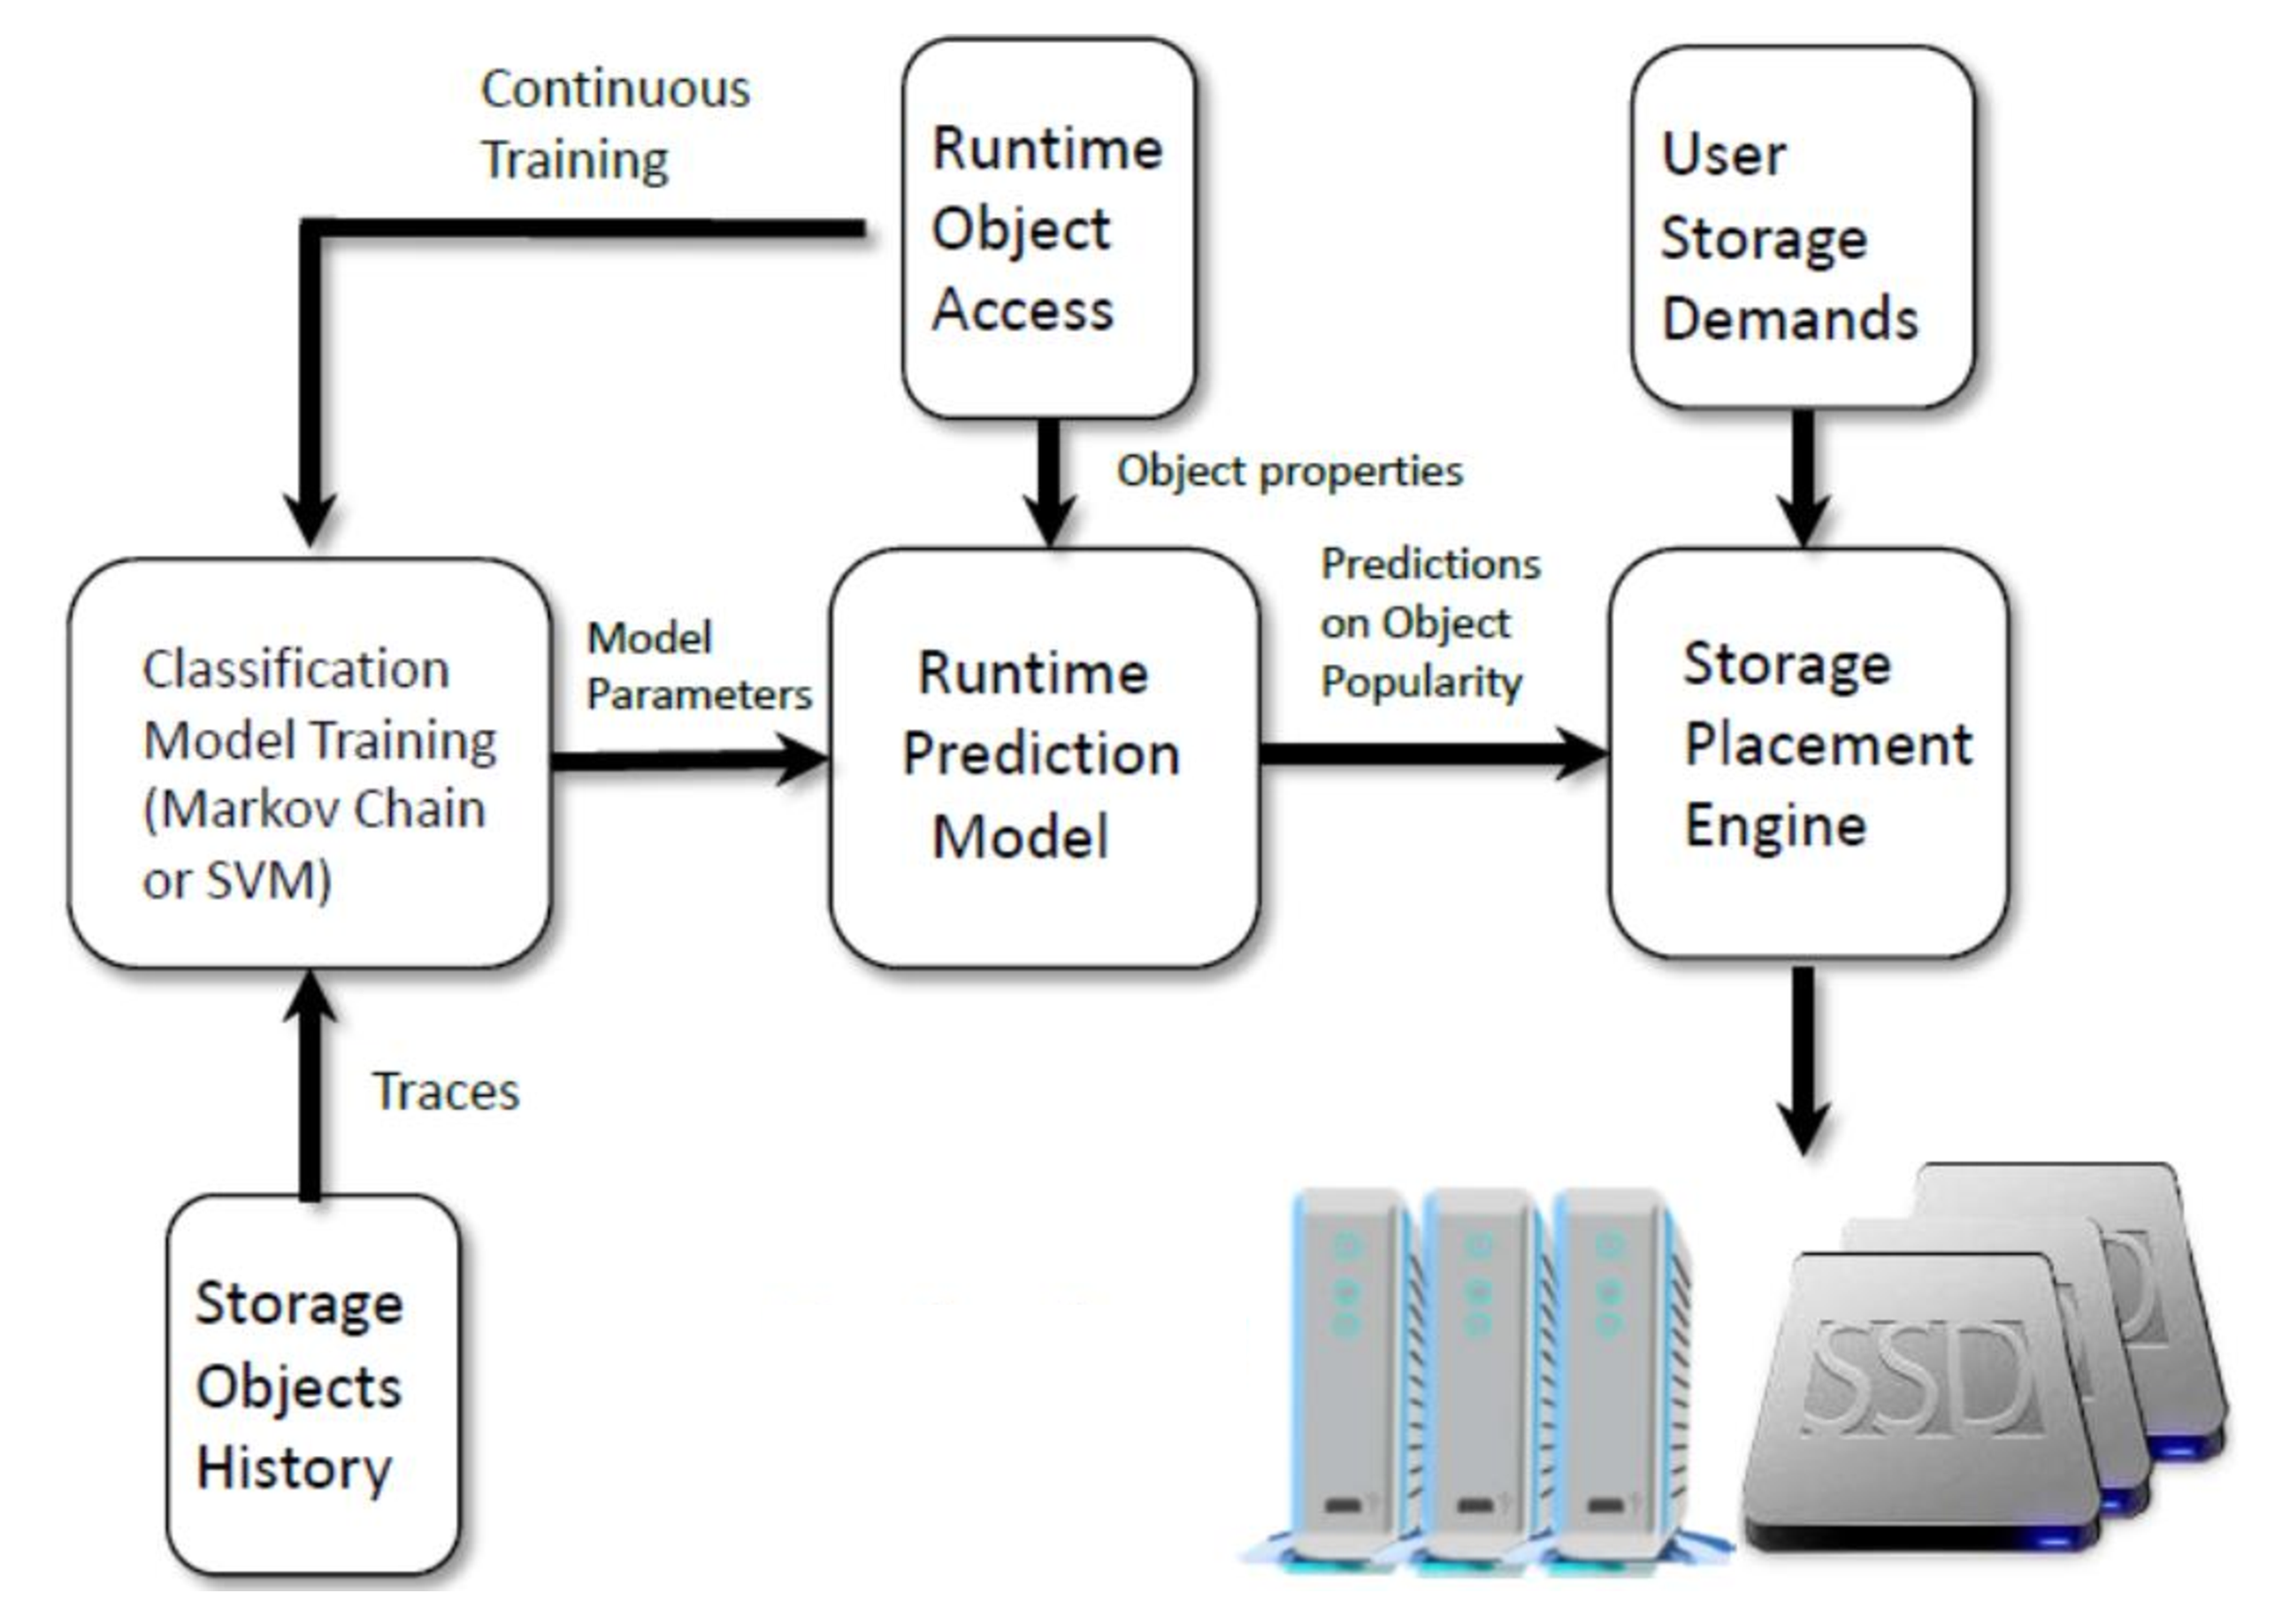
\includegraphics[width=2.3in]{./arch.pdf}
  \caption{The Design Architecture}\label{fig:architecture}
  \label{arch}
\end{centering}
\vspace{-0.1in}
\end{figure}






\subsection{Architecture Overview}
\label{architecture}


We first present the design architecture of our data placement algorithm. For this design, we consider the I/O workload from user applications to include both read and write operations. All I/O workload are generated to access data objects, which are minimal storage units in object-based storage systems. In practice, a large file can be divided into multiple data objects which will be stored on single or multiple object-based storage devices (OSDs). Note that the write operations may be dominating for certain I/O workload, such as periodic checkpoint~\cite{naksinehaboon2008reliability}. The I/O workload from user applications may also change over time, therefore, the solution should adapt to the dynamic nature of the I/O workload.

Figure~\ref{arch} shows the overall architecture, where the whole procedure works as follows: the first core component, the classification model, is trained based on the access history of data objects. In our current work, we concentrate on the historical access frequency of data objects, while we leave exploiting the access pattern (sequential/random read or write) to improve data placement performance as our future work. After training, it provides parameters for the runtime prediction model that are used to predict the access popularity of data objects in the future. Specifically, the predictions decide if an object is going to have ``recurring'' or ``non-recurring'' accesses, based on its history of accesses, as well as the particular workload that accessed them. Such predictions are then used, together with user demands, as the input for the storage placement engine, whose goal is to generate an optimized placement of data objects to storage devices so that the overall system level performance on access delay and bandwidth can be improved. Finally, the runtime object access traces are also used as input for the classification model for continuous training purposes, and keeping the parameters up-to-date.


\subsection{Markov Chain based Workload Classification}

In this section, we describe how the classification model generates model parameters based on object access traces. In our design, we adopt a Markov chain based approach. %Formally, we first select a list of features for a data object for training purposes. Suppose that we select an $N$-tuple that forms a workload signature as:

%\[
%  Signature = {m^1, m^2, ..., m^n}
%\]
%
%where the $m^i$ represents a measured metric of $i$. Note that the metric selection process is fully automated and transparent to the user. The particular $m^i$ may have flexible semantics, and for our present purpose, we focus primarily on its metric of access frequency.

%Once the signatures are collected, it is important that we can classify later workloads based on the training periods. This is based on the assumption that user workloads will have inherent repeating patterns, where similar workloads may be encountered again. This therefore resembles the ``cache hit rates'' which are well studied in the computer cache designs. But still there are considerable differences, as unlike cache contents, the workload signatures may indeed shift over time. Therefore, it is only giving approximate solutions, not accurate answers.

Observe that there exists a tradeoff in the overhead of training and the prediction accuracy. Therefore, we need to achieve a good tradeoff in our design. Our approach has the following key steps. First, we assume that we can keep the access history for each data object. In reality, it may not be practical to record a long access history for each data object since in that case the storage overhead could be huge, instead, only recent access history needs to be maintained and updated periodically. Second, we model the access frequency of each data object using a discrete-time Markov chain in which each state represents a specific range of access frequency. With the access history, we can estimate the parameters of the Markov chain model. Third, by calculating the stationary distribution of the Markov chain, we can predict the likelihood for the access frequency of each data object to stay within certain ranges in the long run. Finally, we rank each data object based on the weighted sum of the stationary distribution, where the weights are chosen according to the specific range represented by each state in the Markov chain. A higher rank of the data object indicates that it is more appropriate and efficient to be moved or placed into low-latency, high-bandwidth drives such as SSDs. We next describe these steps in more detail.

\subsubsection{Collection of Access History of Data Objects}


\begin{figure}[!t]
\centering
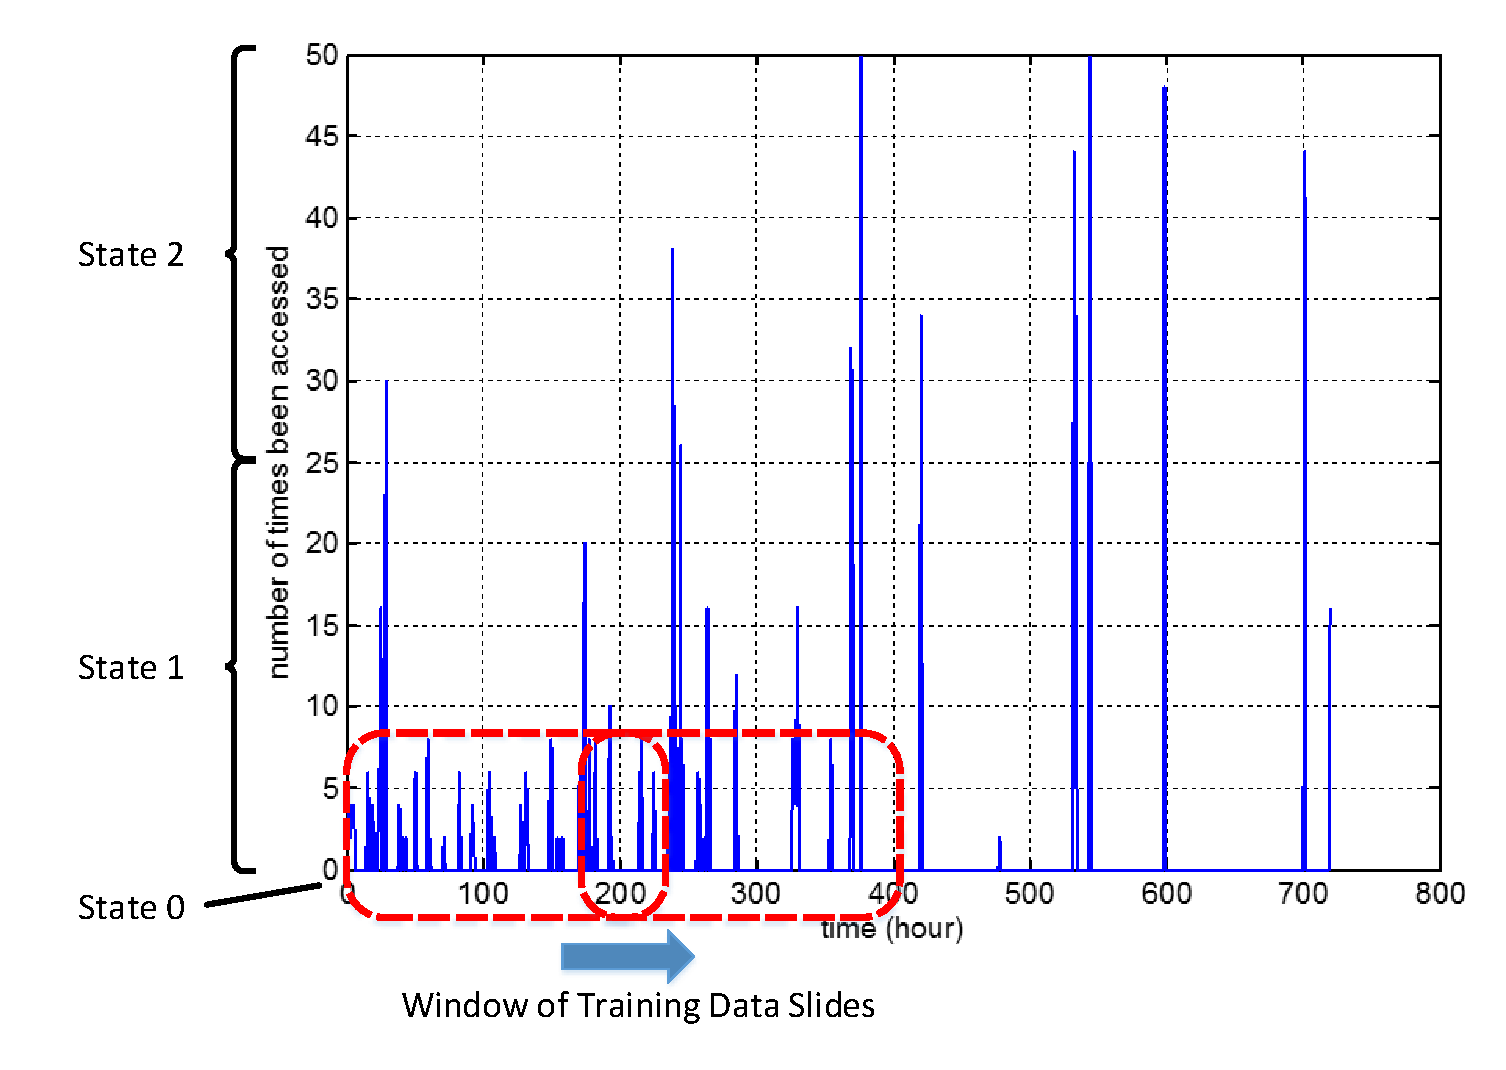
\includegraphics[width=3.0in]{./trace.pdf}
% where an .eps filename suffix will be assumed under latex,
% and a .pdf suffix will be assumed for pdflatex; or what has been declared
% via \DeclareGraphicsExtensions.
\caption{Traces of Data Object Accesses in Frequency}
\vspace{-0.25in}
\label{trace}
\end{figure}


Fig. \ref{trace} demonstrates the access frequency (here the ``access'' includes both read and write operations) of a data object during one month from the LASR traces~\cite{tracedata2}, which include I/O activities of benchmark applications for the SEER project, which observes users' file access patterns across storage networks. The X axis of Fig. \ref{trace} is the range of one month time that has been divided into 720 time periods (each period is 1 hour). The Y axis represents the number of times the data object has been accessed during each time period. As the storage overhead for maintaining the entire access history of each data object is not cost-effective, we only maintain recent access history of each data object and use such access history to build a Markov chain model to predict the future access frequency. As shown in Fig. \ref{trace}, only the access history in the dotted window is used to train the prediction model, where the window will slide with time so that we can implement online prediction for data objects access frequency.

\subsubsection{Markov Chain Predication Model}

With the access history of each data object, we build a Markov chain model to predict the future access frequency of data objects. First, we need to determine how many states the Markov chain should have and the range of access frequency each state represents. For example, as shown in Fig. \ref{trace}, if the maximum number of access times during an observation period is 50, then, for example, we can divide 50 evenly into two ranges, and build a Markov chain model that has three states: $0$, $(0,25]$, and $(25,50]$, respectively. If during a time period, there is no access of the data object, then the Markov chain will stay in state 0. If the number of access times is larger than 0 but less than 25, then the Markov chain will stay in state 1, and so on. The transition diagram of the Markov chain is shown in Fig. \ref{transitioin}.

\begin{figure}[!t]
\centering
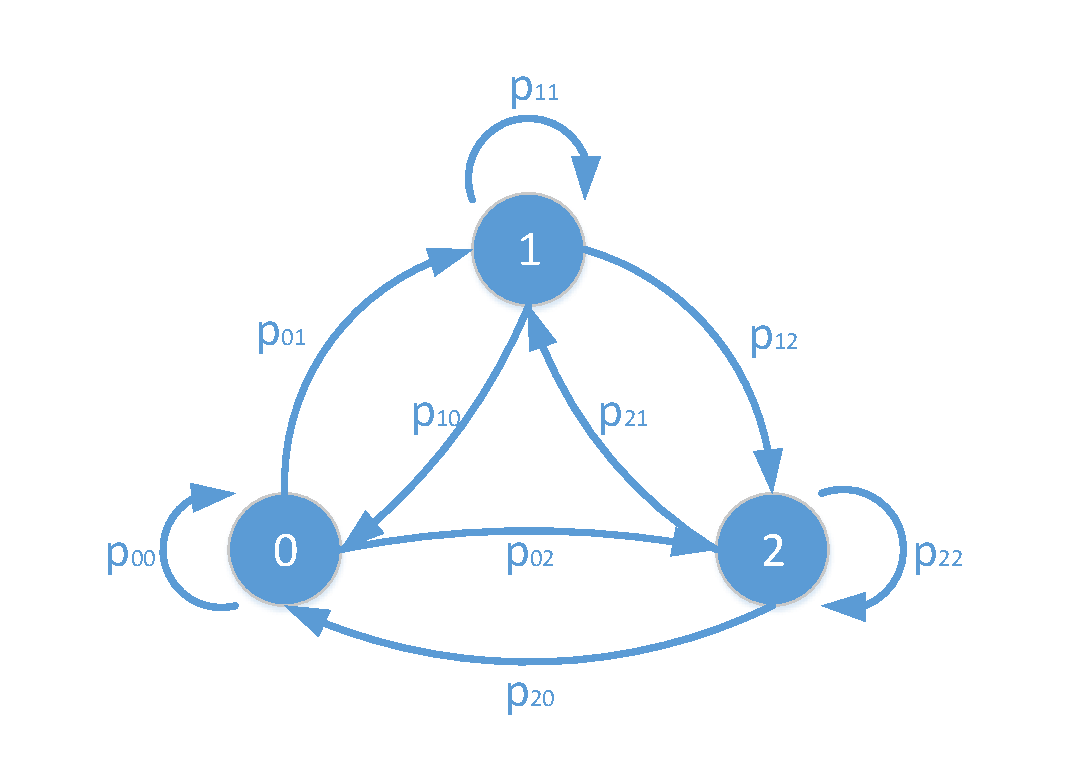
\includegraphics[width=1.9in]{./transition.pdf}
% where an .eps filename suffix will be assumed under latex,
% and a .pdf suffix will be assumed for pdflatex; or what has been declared
% via \DeclareGraphicsExtensions.
\caption{Transition Diagram of Markov Chain}
\vspace{-0.25in}
\label{transitioin}
\end{figure}

Second, we transform the access history to the state transition sequence of the Markov chain based on the specific range each state represents. For example, after transformation the state transition sequence of access history shown in Fig. \ref{trace} is: 1,1,1,1,1,0,0...  Based on this state transition sequence, we can estimate the transition probabilities between every two states and construct the transition matrix of the Markov chain shown below:

\begin{equation}
\mathbf{T} =
 \begin{pmatrix}
  p_{00} & p_{01} & p_{02} \\
  p_{10} & p_{11} & p_{12} \\
  p_{20} & p_{21} & p_{22}
 \end{pmatrix}
\end{equation}

According to the properties of Markov chain, we have:
\begin{equation}
\lim_{n\to\infty}\mathbf{T}^{n} =
 \begin{pmatrix}
  \pi_{0} & \pi_{1} & \pi_{2} \\
  \pi_{0} & \pi_{1} & \pi_{2} \\
  \pi_{0} & \pi_{1} & \pi_{2}
 \end{pmatrix}
\end{equation}
in which $\boldsymbol{\pi} = [\pi_{0}, \pi_{1},  \pi_{2}]$ is called the stationary distribution of the Markov chain. We can simply calculate $\boldsymbol{\pi} $ through computing a normalized multiple of a left eigenvector $\mathbf{E}$ of the transition matrix $\mathbf{T}$ with an eigenvalue of 1:
\begin{equation}
\boldsymbol{\pi} = \frac{\mathbf{E}}{\sum_{i}e_{i}}
\end{equation}
where $e_{i}$ is the $i$-th element of eigenvector $\mathbf{E}$. Since the stationary distribution $\boldsymbol{\pi}$ reflects the probabilities that each state of Markov chain will be visited in the future, which can be used to predict the access frequency of each data object.

Based on the predicted access frequency in the future, we rank the data objects  so that we can determine which data object should be placed or moved to SSD drives. Note that, however, even if the calculated stationary distribution tells us state 1 will be visited with higher probability than state 2, to rank the importance of the data object, we must consider that state 2 represents a higher access frequency. Therefore, we use a weighted sum of the stationary distribution to rank the importance of the data objects, where the weights are defined by values that are proportional to the access frequency ranges that the states represent. For example, if we obtain the stationary distribution of the data object as $\boldsymbol{\pi} = [0.31, 0.56, 0.13]$, and we assign weights $[0, 10, 20]$ to the three different states, we can calculate the rank of the data object by $rank_{obj_{x}} = 0.31\times0+0.56\times10+0.13\times20 = 8.2$. We can then compare the ranks of objects, and provide input for the placement engine.

\begin{table}[t]
\centering
\scriptsize
\begin{tabular}{|l|l|}
\hline
 $N$ & Total number of storage drives \\
 \hline
 $M$ & Total number of data objects  \\
 \hline
 $cs_i$ & Capacity of storage drive $i$ \\
 \hline
 $ds_i$ & Size of data object $i$\\
 \hline
 $f_i$ & Predicted frequency of access for data object $i$\\
 \hline
 $b_{ij}$ & Bandwidth for the link connecting storage drives $i$ and $j$\\
 \hline
 $at_i$ & Average throughput for storage drive $i$\\
 \hline
 $e_{ij}$ & Whether data object $i$ is stored on storage drive $j$ ($0$ or $1$)\\
 \hline
 $cp_i$ & The minimum number of copies for data object $i$\\
 \hline
\end{tabular}
\normalsize
\caption{Notations of Symbols}
\vspace{-0.3in}
\label{tablenotes}
\end{table}


\subsection{Finding Placements under User Polices}

Once we obtain the predicted popularity of data objects, i.e., their ranks, the next step is to find an optimized placement solution such that the access latency is minimized, while satisfying users' placement policies. In this aspect, we assume that users' requests will be parametric, meaning that all requests will be embedded into equations or constraints. For example, by using the notations in Table~\ref{tablenotes}, a requirement on the number of redundant copies of a data object $i$ stating that at least three extra copies must be made can be expressed as $cp_i > 3$.

Our solution to this problem is by formulating the placement problem in a mathematical optimization as follows:

We want to maximize:

\begin{equation}
\sum\limits_{i \in M} f_i \times max[\forall j \in N, at_j\times e_{ij} ]
\label{goalmetric}
\end{equation}

subject to constraints such as:

\begin{equation}
\sum\limits_{j\in N} e_{ij} = cp_i, \forall i \in M,
\label{capacity}
\end{equation}

\begin{equation}
\sum\limits_{\forall i \;\; s.t.\;\; e_{ij} = 1} ds_i \le cs_j, \forall j \in N, \label{duplicate}
\end{equation}

In this short paper, we only give a description of an easier scenario in these equations. In this example, Equation~\ref{goalmetric} specifies that we want to find a way that assigns data objects to storage devices such that the weighted access throughput by the access frequency is maximized.  Note that we use the equation $at_j\times e_{ij}$ to filter those storage devices where the particular data object $i$ is stored on: if $i$ is stored on device $j$, we know $e_{ij}=1$, otherwise $e_{ij}=0$. Hence, finding the $max$ of them translates into finding the storage unit with a copy of data object $i$ that has the highest throughput.

On the other hand, this optimization goal is subject to two or more constraints. In this example, we only consider two of them, in Equation~\ref{capacity} and Equation~\ref{duplicate}, respectively. The first constraint specifies that each storage drive $j$ should not contain more data objects than its capacity, while the second constraint specifies that the number of duplicate copies of a data object should be set according to the users' placement polices. If a data object does not need to have duplicates, its $cp$ value is set to $1$ by default.

In more complex scenarios, the users may have additional constraints. As we mentioned earlier, such constraints are parameterized, meaning that we can easily add more constraints to the formulation above. Finally, even the optimization goal can be adjusted. For example, if we only want to minimize the access delay rather than the throughput, we can change the Equation~\ref{goalmetric} accordingly.

Based on this formulation, we notice that the optimization is reduced to a linear programming problem where we can use numerical methods to recalculate its solution periodically in the placement engine. Note that the engine is operating independently of the rest of the system. Doing so does not require the engine to be tightly integrated, so that we can easily change the engine's implementation as needed, which gives us additional flexibility.


%\section{Analytical Modeling of Algorithm Performance}
\label{analysis}

In this section, we model the system performance using analytic approaches. 

\section{System Evaluation}
\label{sec:evaluation}

\begin{figure}[!t]
\centering
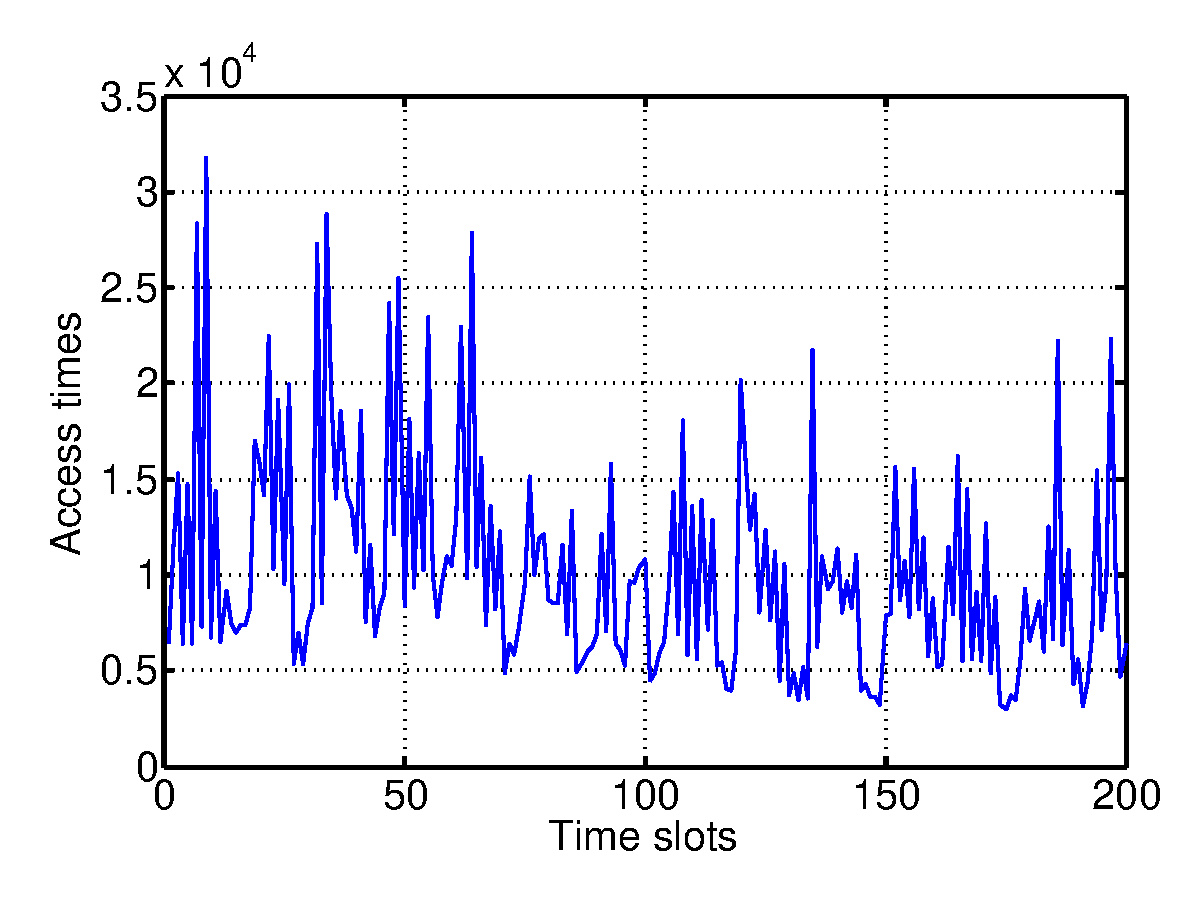
\includegraphics[width=2.0in]{./datafig1.pdf}
% where an .eps filename suffix will be assumed under latex,
% and a .pdf suffix will be assumed for pdflatex; or what has been declared
% via \DeclareGraphicsExtensions.
\caption{Illustration of Data Access Traces Type I}
\vspace{-0.1in}
\label{datafig1}
\end{figure}

\begin{figure}[!t]
\centering
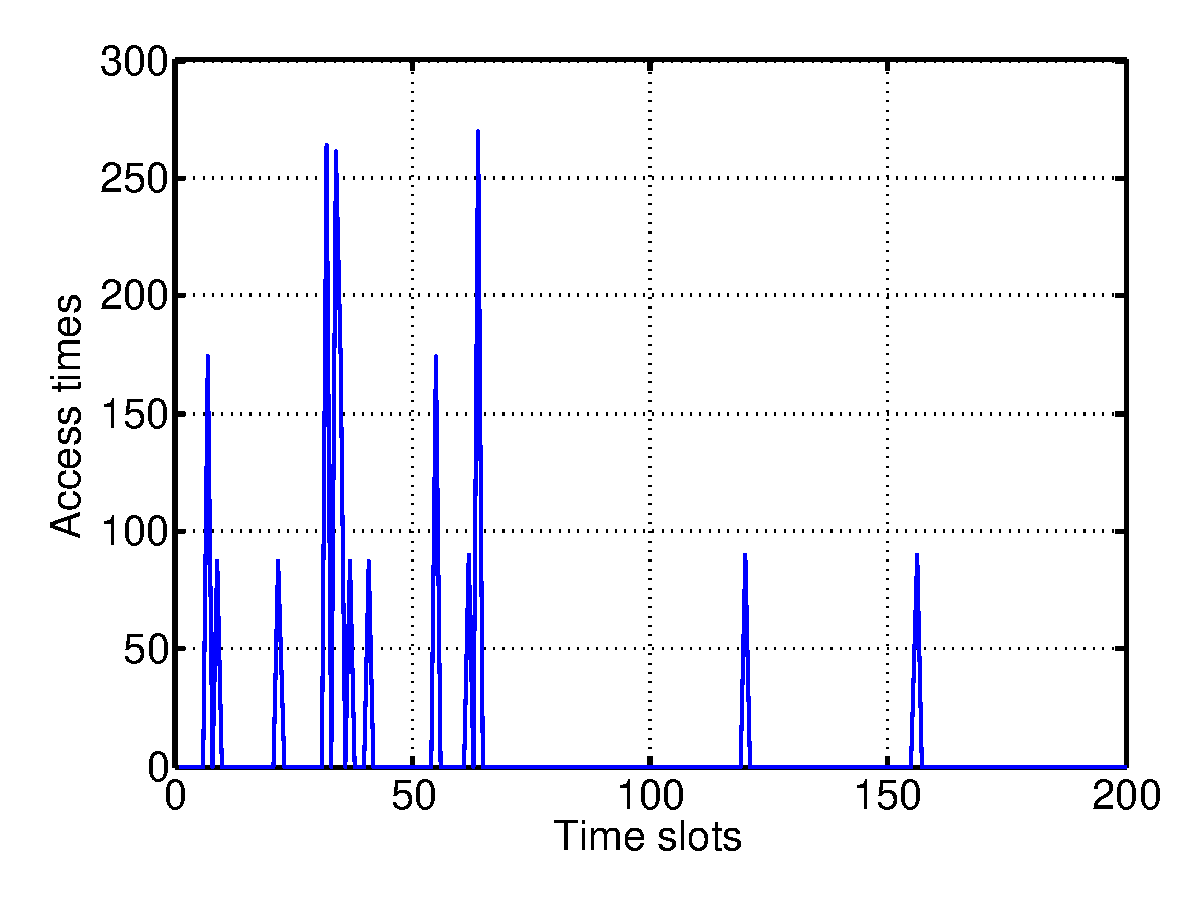
\includegraphics[width=2.0in]{./datafig2.pdf}
% where an .eps filename suffix will be assumed under latex,
% and a .pdf suffix will be assumed for pdflatex; or what has been declared
% via \DeclareGraphicsExtensions.
\caption{Illustration of Data Access Traces Type II}
\vspace{-0.25in}
\label{datafig2}
\end{figure}


In this section, we systematically present the evaluation of the proposed algorithm. We first present a study of the traces of data object accesses, based on which we evaluate the performance of our learning algorithm by replaying them. We use a long-term I/O traces, LASR traces~\cite{tracedata2}, which were collected at system-call level. We track the access frequency of different files during their lifetime. Specifically, we divide the time span into hundreds of time slots and each of which has same length. We then count how many times each file has been accessed during each time slot. In the LASR traces, we eliminate those files which have only been accessed less than 10 times during their lifetime (the access of these files almost has no impact on the performance of the storage system) and focus on the remaining ones (1,703 files) which are more frequently accessed. By analyzing the access of these frequently accessed files, we find out that these files can be roughly put into two categories according to their access patterns. The first category contains files that have constant access patterns. Files in this category have been frequently accessed during their whole lifetime, without too much difference between the maximum and minimum access periods. Fig.~\ref{datafig1} shows a typical file falls into this category. The learning algorithm, especially the Markov chain approach can achieve a higher level of accuracy for this kind of files. The second category is files with a bursty access pattern. Files in this category have only been accessed at very few time slots, but the access counts for those time slot can be very large. Fig.~\ref{datafig2} shows a typical file falling into this category. For files belong to second category, it is pretty hard for any learning algorithm including Markov chain approach to train a model to accurately predict their future access frequency.


To save the evaluation time, we did not use the entire LASR traces, instead, from the dataset we select traces of files that have been accessed more than 1,000 times (traces of 40 different files). For each trace we use the first half as the training data to train our Markov prediction model while use the other half as the testing data. As illustrated in Fig. \ref{prediction}, the bars represent the future access frequency of the 40 different files which are extracted from the testing dataset. Since we only have limited SSD storage space, our goal is to store the files that will be most frequently accessed in the future on SSD devices to improve the average data access throughput. For example, if we can only put 10 of 40 files on SSDs, as shown in Fig. \ref{prediction}, the light-colored bars illustrate the files predicted by our Markov model that are required to be placed on SSD devices. From the results we can observe that, 7 of 10 files that have the highest future access frequency have been chosen.

\begin{figure}[!t]
\centering
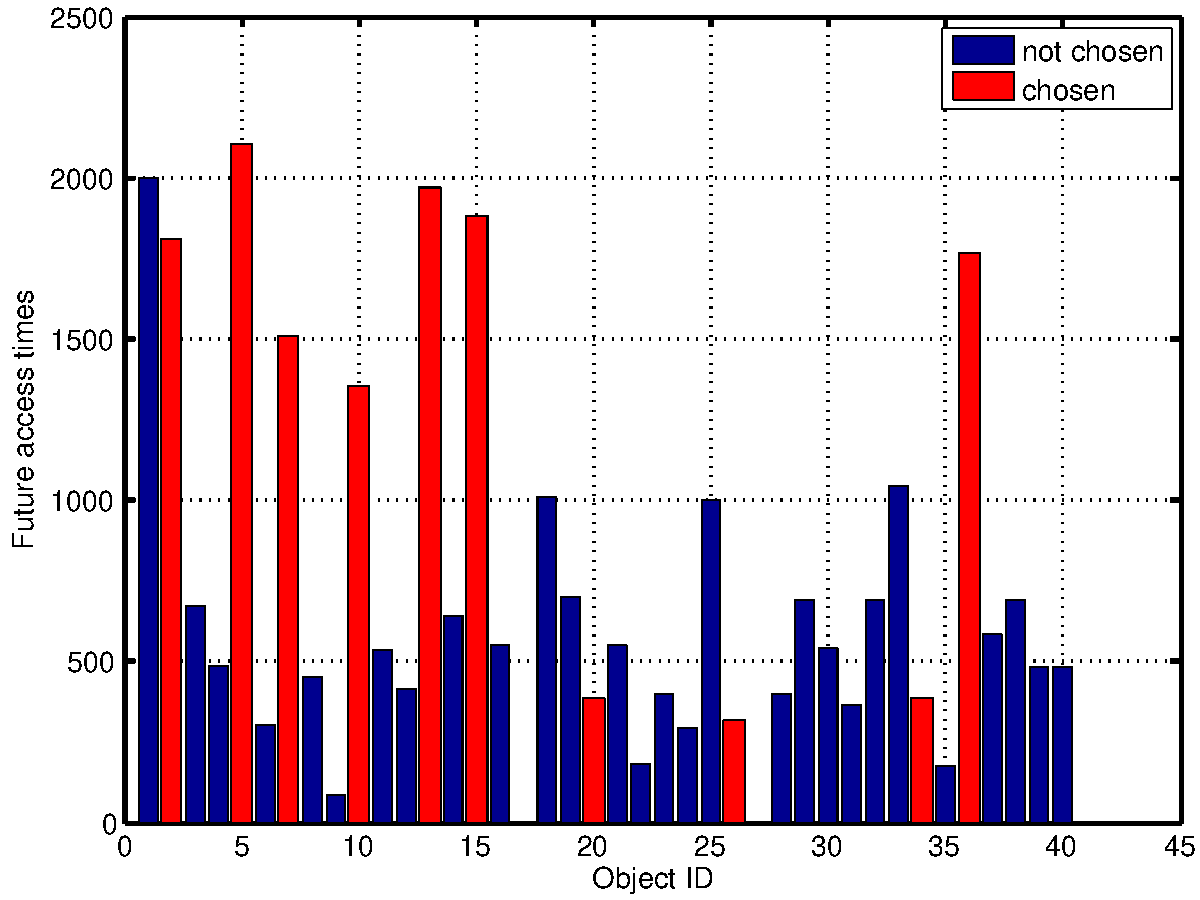
\includegraphics[width=2.4in]{./prediction.pdf}
% where an .eps filename suffix will be assumed under latex,
% and a .pdf suffix will be assumed for pdflatex; or what has been declared
% via \DeclareGraphicsExtensions.
\caption{Future Access Times of Data Objects}
\vspace{-0.1in}
\label{prediction}
\end{figure}

\begin{figure}[!t]
\centering
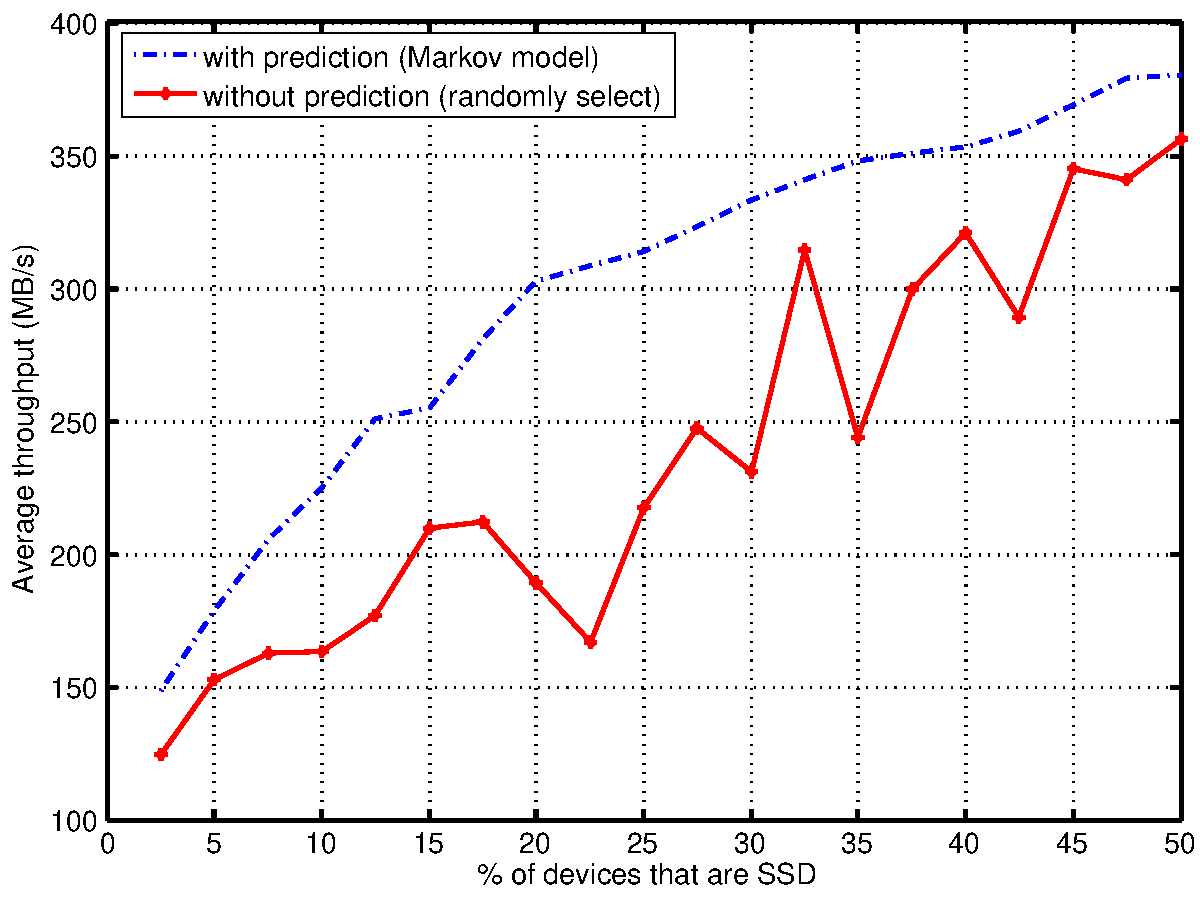
\includegraphics[width=2.4in]{./throughput.pdf}
% where an .eps filename suffix will be assumed under latex,
% and a .pdf suffix will be assumed for pdflatex; or what has been declared
% via \DeclareGraphicsExtensions.
\caption{Average Throughput v.s. Percentage of Objects Stored on SSDs}
\vspace{-0.25in}
\label{throughput}
\end{figure}

We next choose random selection approach as baseline and compare the average read throughput achieved by our Markov prediction model with that achieved by random object selection. Here the random object selection means that we randomly choose several data objects (files) and put them on SSD devices. The number of data objects that can be placed on SSD devices is also limited. For example, in the simulation, we vary the number of data objects that can be put on SSD devices from 2.5\% to 50\%. Besides, we set the read throughput of SSD devices as 550MB/s and that of HDD devices as 120 MB/s, consistent with typical datasheets provided by manufacturers of storage devices \cite{chen2009understanding}. As shown in Fig. \ref{throughput}, our object selection approach can achieve higher average read throughput than random selection, demonstrating the effectiveness of our proposed approaches.



%\section{Application Case Study}
\label{casestudy}

\subsection{Problem Overview}

Describes the workload problem

\subsection{Details}

Describes the details of the implementation for this application case study. 
\section{Conclusions}
\label{sec:conclusion}

In this paper, we presented a study of developing a hybrid configuration (SSD and HDD) for storage needs of HPC environments. Specifically, we proposed an integrated object placement framework with adaptive learning algorithms. The method placed data objects with considering both the popularity of the data and the capability of different storage devices, so that the data access performance can be optimized. The method also integrated a Markov chain algorithm where real-time classification is employed to predict the popularity of data object accesses, so that they can be placed on, or migrate between SSD or HDD drives in the most efficient manner. Our preliminary results based on realistic data traces demonstrate that this approach is highly promising, and achieves better performance than benchmark methods such as pure random selections.

\section{Acknowledgement}
\label{acknowledgement}
We would like to thank the anonymous reviewers for their insightful comments. The work reported in this paper was sponsored by the Laboratory Directed Research and Development Program of Oak Ridge National Laboratory, managed by UT-Battelle, LLC, for the U.S. Department of Energy, and by the National Science Foundation grant 0953238.


{\tiny
\bibliographystyle{IEEEtran}
\bibliography{reference}
}

\end{document}
